\documentclass[twoside,a4paper,12pt]{report}
\usepackage{graphicx}
\usepackage{amsmath}
\usepackage{appendix}
\usepackage{nameref}
\usepackage{float}
\usepackage{flafter}
\usepackage{url}
\def\UrlBreaks{\do\/\do-}
\Urlmuskip=0mu plus 1mu
\usepackage[
backend=biber,
style=alphabetic
]{biblatex}
\setcounter{biburllcpenalty}{7000}
\setcounter{biburlucpenalty}{8000}
 \usepackage[T1]{fontenc} 
 \usepackage[final]{microtype}
\emergencystretch=1em
\graphicspath{ {images/} }
\usepackage[utf8]{inputenc}
\usepackage[spanish,english]{babel}

\usepackage[table]{xcolor}% http://ctan.org/pkg/xcolor


\usepackage{titlesec}

\setcounter{secnumdepth}{4}

\titleformat{\paragraph}
{\normalfont\normalsize\bfseries}{\theparagraph}{1em}{}
\titlespacing*{\paragraph}
{0pt}{3.25ex plus 1ex minus .2ex}{1.5ex plus .2ex}
 
\setlength{\parindent}{4em}
\setlength{\parskip}{1em}
\renewcommand{\baselinestretch}{1.3}

\usepackage{indentfirst}

\usepackage{mathptmx}


\usepackage{listings}
\usepackage{xcolor}
 
\definecolor{codegreen}{rgb}{0,0.6,0}
\definecolor{codegray}{rgb}{0.5,0.5,0.5}
\definecolor{codepurple}{rgb}{0.58,0,0.82}
\definecolor{backcolour}{rgb}{0.95,0.95,0.92}
 
\lstdefinestyle{mystyle}{
    backgroundcolor=\color{backcolour},   
    commentstyle=\color{codegreen},
    keywordstyle=\color{magenta},
    numberstyle=\tiny\color{codegray},
    stringstyle=\color{codepurple},
    basicstyle=\ttfamily\footnotesize,
    breakatwhitespace=false,         
    breaklines=true,                 
    captionpos=b,                    
    keepspaces=true,                 
    numbers=left,                    
    numbersep=5pt,                  
    showspaces=false,                
    showstringspaces=false,
    showtabs=false,                  
    tabsize=2
}
 
\lstset{style=mystyle}



\graphicspath{ {images/} }

\usepackage[]{geometry}
 \geometry{
 a4paper,
 total={170mm,257mm},
 inner=25mm,
 outer=25mm,
 top=25mm,
 bottom=25mm
 }
 
 



\usepackage{csquotes}

\addbibresource{references.bib}

\usepackage{titlesec}

\titleformat{\paragraph}
{\normalfont\normalsize\bfseries}{\theparagraph}{1em}{}
\titlespacing*{\paragraph}
{0pt}{3.25ex plus 1ex minus .2ex}{1.5ex plus .2ex}
 
\setlength{\parindent}{4em}
\setlength{\parskip}{1em}
\renewcommand{\baselinestretch}{1.3}

\usepackage{indentfirst}

\usepackage[]{geometry}
 \geometry{
 a4paper,
 total={170mm,257mm},
 inner=25mm,
 outer=25mm,
 top=25mm,
 bottom=25mm
 }
 
% \title{Machine learning and pattern recognition project}
\usepackage{csquotes}

\title{Machine Learning Project}
\author{
    Simone Grimaldi S260770 \\
Alfredo Baldó Chamorro     S288347\\}
\begin{document}

\maketitle
\tableofcontents

\newpage
\newpage


\setcounter{chapter}{1}


\section{Dataset}

The dataset contains the information of red and white variants of the Portuguese "Vinho Verde" wine. 
It has been split into Test and Train sets containing 1822 and 1839 samples respectively. 
Moreover, there are two classes: good quality (value 1) and bad quality wine (value 0), 
where each has twelve attributes. Moreover, the table \ref{RangeAndTypesAttributes} 
resumes the information related to the attributes.

\begin{enumerate}
    \item fixed acidity
    \item volatile acidity
    \item citric acid
    \item residual sugar
    \item chlorides
    \item free sulfur dioxide
    \item total sulfur dioxide
    \item density
    \item pH
    \item sulphates
    \item alcohol
\end{enumerate}



\begin{table}
\centering
 \begin{tabular}{||c c c||} 
 \hline \hline
 Attributes & Range & Type\\ 
 \hline\hline
 Fixed acidity & [3 ; 15.9] & Continuous\\ 
 \hline
 Volatile acidity & [0.1 ; 1.58] & Continuous\\
 \hline
 Citric acid & [0 ; 1] & Continuous \\
  \hline
 Residual sugar & [0.7 ; 23.5] & Continuous \\
  \hline
 Citric acid & [0 ; 1] & Continuous \\
 \hline
 Chlorides & [0.013 ; 0.611] & Continuous \\
 \hline
 Free sulfur dioxide & [2 ; 289] & Continuous \\
 \hline
 Total sulfur dioxide & [7 ; 440] & Continuous \\
  \hline
 Density & [0.9874 ; 1.0032] & Continuous \\
  \hline
  pH & [2.79 ; 3.9 ] & Continuous \\
   \hline
 Sulphates & [0.25 ; 1.36] & Continuous \\
  \hline
 Alcohol & [8 ; 14.9] & Continuous \\
  \hline
 Total sulfur dioxide & [7,440] & Continuous \\
 \hline \hline
\end{tabular}
\caption{Range and types of the attributes \label{RangeAndTypesAttributes}
}
\end{table}


\begin{figure}
    \centering
    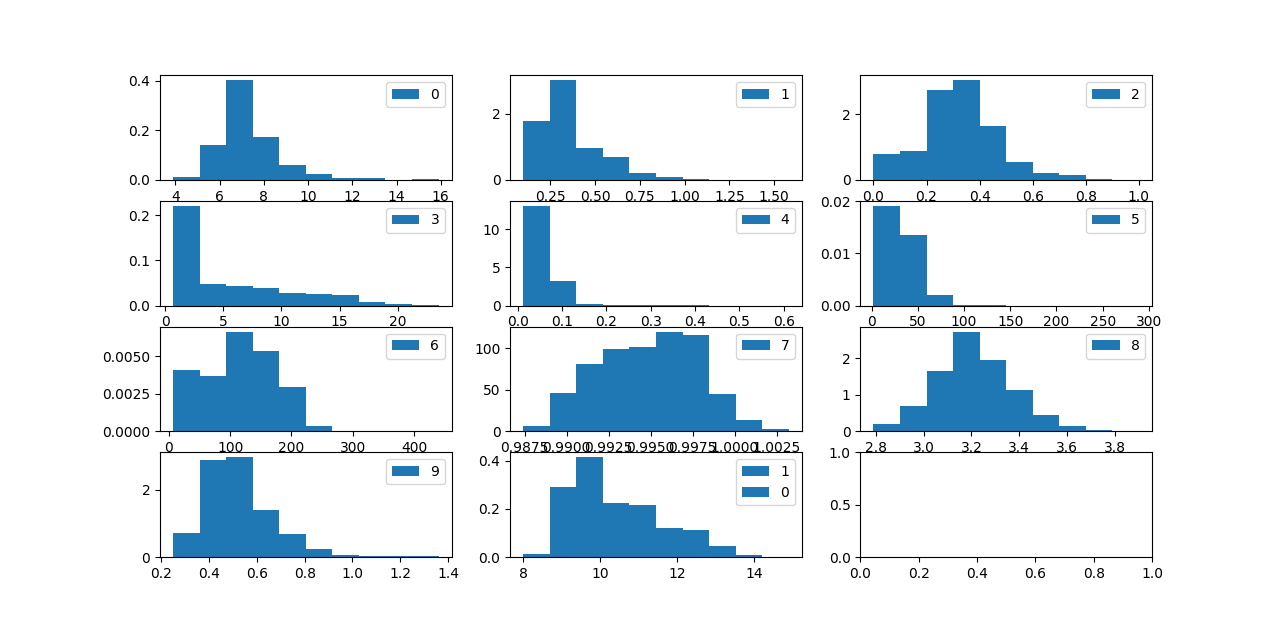
\includegraphics[width=1\textwidth,height=0.7\textheight]{histograms.png}
    \caption{Histograms of the attributes (numerated) without modification}
     \label{HistogramsWithoutMod} 
\end{figure}

\subsection{Correlations}
The range of the each attribute is stated in the table \ref{RangeAndTypesAttributes}.
Moreover, the image \ref{CorrelationRaw} illustrates the correlation between the attributes in the dataset. 
It can be extracted from the figure that the most correlated attributes are (7,10), (6,5) (6,3) and 
(7,3) (see table \ref{ResumeCorrelation}).  Even though the correlation is higher in those attributes,
 the values are still unimportant (lower than 0.8) in order to consider a strong correlation between them.



\begin{figure}
    \centering
    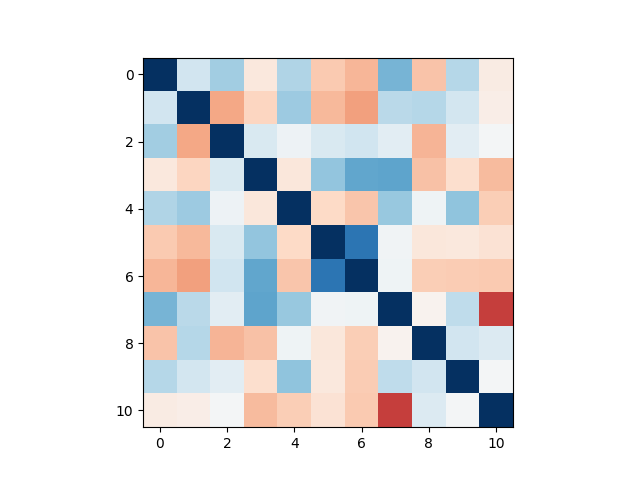
\includegraphics[width=1\textwidth,height=0.5\textheight]{correlation_no_transformation.png}
    \caption{Correlations of the raw data (Pearson's coefficient)}
     \label{CorrelationRaw} 
\end{figure}

\begin{table}
    \centering
    \begin{tabular}{|| c|c|c||}
          \hline \hline
         Attributes (by pairs) & Tag & Correlations  \\
         \hline \hline
         (7,10) & (density, alcohol) & -0.692\\
         \hline
         (6,5) & (total sulfur dioxide, free sulfur dioxide) & 0.73  \\
         \hline
         (6,3) & (total sulfur dioxide, residual sugar) & 0.52 \\
         \hline
         (7,3) & (density, residual sugar) &0.526 \\
         \hline  \hline
    \end{tabular}
    \caption{Most correlated attributes     \label{ResumeCorrelation}
    }
\end{table}




\subsection{PCA - Principal Component Analysis}

Principal Component Analysis or PCA is a widely used technique for dimensionality 
reduction of the large data set. Reducing the number of components or features costs
 some accuracy and on the other hand, it makes the large data set simpler, easy to 
 explore and visualize. Also, it reduces the computational complexity of the model 
 which makes machine learning algorithms run faster.

% \subsection{Use PCA on our dataset}
\textbf{Steps Involved in PCA}
\begin{enumerate}
    \item Standardize the data (with mean =0 and variance = 1).
    \item Compute the Covariance matrix of dimensions.
    \item Obtain the Eigenvectors and Eigenvalues from the covariance matrix
    \item Sort eigenvalues in descending order and choose the top k Eigenvectors 
    that correspond to the k largest eigenvalues (k will become the number of 
    dimensions of the new feature subspace k $\leq$ d, d being the number of original dimensions).
    \item Construct the projection matrix W from the selected k Eigenvectors.
    \item Transform the original data set X via W to obtain the new k-dimensional feature subspace Y.
\end{enumerate}

Analyzing the eigenvalues obtained,  we extracct from figure \ref{PCAChosenComponents} how almost all of the information
can be obtained using 4 or 5 dimensions.
By drawing the cumulative graph of the eigenvalues, the same conclusion can be extracted.
Hence, PCA could be implemented and see if the accuracy improves significantly.
\begin{figure}[H]
    \centering
    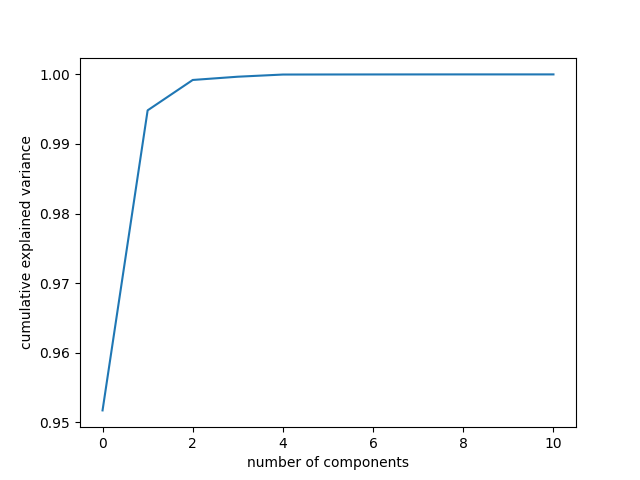
\includegraphics[width=0.7\textwidth,height=0.4\textheight]{cumulative_explained_variance.png}
    \caption{Cumulative explained variance according to the number of components after PCA     \label{PCAChosenComponents} 
    }
\end{figure}


\section{Classifiers}
In order to perform the classification, we have performedd cross validation on the 
training set with k = 8.
The decision for that value of k was taken due to one major factor: time. In fact, the size of the sample being 
1839, the leave-one-out method was discarded due to time needed to perform it.
Moreover, while performing k-fold with some classifiers, k = 8 appeared as an affordable value 
concerning time consumption, whilst performing a decent classification (> 80\%).
Hence every time the k-fold is performed, we are using k = 8 unless stated otherwise.

\subsection{Generative models}

In order to classify the data, different genereative models have been taken into account:
mutlivariate gaussian classifier, tied covariance, Naive Bayes through a k-fold approach including a PCA approach.
 The results are shown in the table \ref{diffTypesclass}. 

 The precision of the models seems to be similar, however the Multivariate  model has a
 greater precision so far with 81.4 \% with PCA, and Naive Bayes performs the worst with 76 \% (without PCA). 
 The explanation of the sligh worse performance of Naive Bayes  can be due to the fact that when we 
 perform the diagonalization of the covariances, we do so by putting zero in the other elements
  of the matrix, hence inevitably losing information. 

 So far, from the table it can be extracted that the MVG classifier with PCA is so far the best solution with
  a 81.4 \% accuracy.

\begin{table}[H]
\centering
 \begin{tabular}{||c c c||} 
    \hline \hline
    Classifier & Accuracy (\%) & Accuracy with PCA (\%)\\
    \hline\hline
    Multivariate & 80.3 & \cellcolor{blue!25} 81.4  \\ 
    \hline
    Tied Covariance & 79 & 79.7  \\
    \hline
    Naive Bayes & 76 & 79.7 \\
    \hline \hline
\end{tabular}
\caption{Different types of classifiers and their accuracy\label{diffTypesclass}
}
\end{table}


\subsection{Logistic regression}
For the logistic regression model we used  a k-fold approach (k =8), where in each 
one we changed the value of lambda. The values of lambda tested where: 
[1e-05, 0.0001, 0.0002, 0.0004, 0.0006, 0.001, 0.004, 0.01]. 
This was done in order to try to get the best model possible.
 This approach was performed with PCA too.
The results are shown in table \ref{errorRateslinearregression}.


As the results in the table \ref{errorRateslinearregression}, the linear regression
without PCA, performed overall better than the model with the PCA.
The best performance of the PCA model was with lambda = 0.0004 
resulting in an error rate of 16.6. The model without PCA, outperforms the model 
with PCA, with its best error rate being 14.4\% (see value in blue).

\begin{table}
    \centering
     \begin{tabular}{||c c c ||} 
        \hline \hline
        lambda & PCA error rate (\%) & no PCA error rate(\%)\\
        \hline\hline
        1.e-5  & 18.34  & 18.8   \\ 
        \hline
        0.0001 & 19.21  &  17.5  \\ 
        \hline
        0.0002 & 20.1  &  14.8  \\ 
        \hline
        0.0004 & 16.6  &  \cellcolor{blue!25}  14.4  \\ 
        \hline
        0.006  & 24.9  & 21    \\ 
        \hline
        0.001  & 22.3  &  18.3  \\ 
        \hline
        0.004 & 20.5  &  20.5  \\ 
        \hline
        0.01  &  18.8 & 15.7   \\ 
        \hline \hline
    \end{tabular}
    \caption{Error rates in (\%) for linear regression with (and without) PCA     \label{errorRateslinearregression}
    }
    \end{table}


\subsection{Confusion matrix and Optimal Bayes}
Concerning the confusion matrix classification model, it has also been performed 
using PCA and without PCA, each done with a k-fold = 8.
We have also take into account a prior of 0.5 for each class. By trying other priors
the precision diminished, therefore we decided to stick with a prior of 0.5. 
Additionally, we decided to put a cost for a false positive of 2 (CFP = 2), while a cost
for a false negative (CFN = 1). This decision was taken as we considered
that missclassifying a "bad" quality wine is worse than missclassifying a 
good quality wine.


The results of computing the optimal Bayes decisions for the parameters previously chosen,
are in the table \ref{errorRatesConfusionMatrix}. As it can be extracted from the table,
using PCA results in a worse performance the raw data inn every classifier except for the
Naive Bayes (with PCA 80.8 \% of precision versus 77.91 \%). 
Finally, the best model seems to be MVG with a precision of 85.5\% and a DCF normalized
of 0.432 (which is the best among the 3 models), which means that implementing the model has 
a positive impact in the classification.


\begin{table}[H]
    \centering
     \begin{tabular}{||c c c c||} 
        \hline \hline
        Classifier & Tied & MVG  & Naive \\
        \hline\hline
        Precision (\%) &  81.86 & \cellcolor{blue!25}  85.5 & 77.91  \\ 
        \hline
        Precision (PCA)  &  79.2 &  80.55 & 80.8 \\ 
        \hline
        DCF &  0.274 &  0.216 & 0.286  \\   
        \hline
        DCF (PCA)  &  0.312 &  0.291 & 0.33  \\   
        \hline
        DCF normalized &  0.548 &\cellcolor{blue!25}  0.432 & 0.572  \\ 
        \hline
        DCF normalized (PCA)  &  0.624 &  0.582 & 0.662    \\ 
        \hline \hline
    \end{tabular}
    
    \caption{Precision in (\%) for different logistic regression models \label{errorRatesConfusionMatrix}}
\end{table}


\subsection{SVM}

We have performed the linear SVM with raw data and with PCA. The results
with PCA underperform the ones with raw data: the best error rate with PCA being
17.9 \% and without PCA 14.4 \% (check results in tables \ref{errorRatesLinearSVM} and \ref{errorRatesLinearSVMNoPCA} respectively).

However, the duality gap for the 17.9 \% error rate for PCA data is 119.13. This
value stands out among the others as really elevated . This could make us think 
that the reliability of the error rate obtained for c = 0.5 can be questioned.

On the other side, the raw data performed well for c = 0.04 and c = 0.05
with both error rates being equal to 14.4 \% while the duality gap being 0
 (check table \ref{errorRatesLinearSVMNoPCA} for results).

After performing linear SVM and having some satisifying results with the 
classification, we decided not to proceed with the kernel SVM due to the high
computational time that took to perform the linear SVM.

\begin{table}[H]
    \centering
     \begin{tabular}{||c c c c||} 
        \hline \hline
            	 c 	& error rate &	 duality gap &	 primal \\ 
                 \hline
            	0.001	&   29.3 &	 0.0 	& 1.122 \\
                \hline
            	0.005 &   24.5 	& 0.0 &	 5.938 \\
                \hline
            	0.01	&   26.2 	 &0.0884 	& 13.15 \\
                \hline
            	0.05	&   30.1 	& 43.1	& 110.63 \\
                \hline
            	0.08	&   25.3 &	 6.11 &	 119.76 \\
                \hline
            	0.1	    &   23.14 	& 3.78	& 157.19 \\
                \hline
            	0.5	&    \cellcolor{blue!25} 17.9	& \cellcolor{red!25} 119.13	& 859.1 \\
                \hline
             	0.9	&   27.1 	& 342.73 	& 1057.13 \\
        \hline \hline
    \end{tabular}
    \caption{Error rate in (\%) for different parameters in linear SVM with PCA \label{errorRatesLinearSVM}}
\end{table}    


\begin{table}[H]
    \centering
     \begin{tabular}{||c c c ||} 
        \hline \hline
            c& error Rate& duality gap \\
            \hline \hline
            0.001&29.7& 0 \\
            \hline
            0.004&20.5& 0.0056\\
            \hline
            0.005& 21.8& 0\\
            \hline
            0.006& 20.1& 0\\
            \hline
            0.007& 16.6& 0\\
            \hline
            0.008& 27.5& 0.0013\\
            \hline
            0.009& 20.5& 0.0001\\
            \hline
            0.01& 17.5& 0\\
            \hline
            0.02&19.2& 0\\
            \hline
            0.03& 17.9& 0.0295\\
            \hline
            0.04& \cellcolor{blue!25}14.4& 0.014\\
            \hline
            0.05& \cellcolor{blue!25}14.4& 0\\
            \hline
            0.06& 21& 5.095\\
            \hline
            0.08& 24.9& 1.645\\
            \hline
            0.1& 19.2& 0.586\\
            \hline
            0.5& 31.9& 2259.61\\
            \hline
            0.9& 18.8& 97\\
\hline \hline
    \end{tabular}
    \caption{Error rate in (\%) for different parameters in linear SVM without PCA \label{errorRatesLinearSVMNoPCA}}
\end{table}    






\subsection{Gaussian mixture models}
For this classsifiers we decided to choose as parameters alpha = 0.1, minimum value
for the eigen vector 0.1. Moreover, we tested until gmm = 16 (1,2,4,8 and 16).

The choice for this parameters was based on the laboratory 10. Once the results appeared,
we didn't change the parameters due to the fact that the results were satisfying (see table \ref{errorRatesGMMs})
and that the computation for every case was too big to repeat. Hence, having
decent precision results we estimated that the the recomputation was not worth the 
possibility of improvement.

The results shown in table \ref{errorRatesGMMs}, illustrate that there is a tendency 
when increasing the model's precision by augmenting the gmm (gmm =16 is the most precise model
in every scenario), this could be due to overfitting as the error rate of this 
method outperforms other models so far (9\% against around 15\% for other models).
 On one hand, the most precise model is the full covariance classifier with PCA previously computed,
resulting in a 9.31\% error rate, versus 9.71 \% without PCA. On the other hand, with a lower complexity (gmm = 8),
the precision is still good enough for the full covariance without PCA (11.8 \%).


\begin{table}[H]
    \centering
     \begin{tabular}{||c c c c c c c c||} 
        \hline \hline
        Classifier & gmm = 1 & gmm = 2 & gmm = 4 & gmm = 8 &gmm = 16 & PCA & k-fold\\
        \hline\hline
        Full covariance &  16.4 &  15.7 &  15.4 & \cellcolor{blue!25}  11.8 & \cellcolor{blue!25} 9.71 & No & 8  \\ 
        \hline
        Full covariance &  17 &  15.8 &  15.8 &  12.9 & \cellcolor{blue!25} 9.31 & Yes & 4  \\ 
        \hline
        Tied Covariance &  16.4 &  16.4 & 16.4 &  16.4 & 14.9  & No & 8  \\
        \hline
        Tied Covariance &  18.6 &  18.6 & 19 &  18.4 & 17.6  & Yes & 8  \\
        \hline
        Diagonal covariance  &  22 &  21.6 & 19.2 &  15.1 & 13.5  & No & 8 \\
        \hline
        Diagonal covariance &20.3 &  21.3 & 21.3&  16.8  & 16 & Yes & 8\\
        \hline \hline
    \end{tabular}
    \caption{Error rates in (\%) for different GMM model classification    \label{errorRatesGMMs}    }
\end{table}

    

\section{Model choice and results}
With all the previously models taken into account, basing ourselves solely 
in the classification performance, what appears to be best at
classifying the data is the GMM model , specifically for gmm =16 with a full covariance and PCA applied.

However, with a punctual classification performance does not mean that the model
will classify better the test data. In fact, with gmm = 16 it appears as 
the model is overfitting itself to the training data.Therefore, considering 
only one performance doesn't appear to be the best decision. The table \ref{errorRatesModels}
takes the best classification result for every classifier.

\begin{table}[H]
    \centering
     \begin{tabular}{||c c ||} 
        \hline \hline
        Classifier & error Rate (\%) \\
        \hline\hline
        GMM = 16 without PCA &  9.71   \\ 
        \hline
        GMM = 8 without PCA &  11.8  \\ 
        \hline
        GMM = 16 with PCA &  9.31    \\
        \hline
        Logistic regression (c = 0.0004 ) &  14.4   \\
        \hline
        MVG (with PCA)  &  18.6 \\
        \hline
        Optimal Bayes (MVG) & 14.5  \\
        \hline
        Linear SVM (c = 0.04)& 14.4  \\
        \hline \hline
    \end{tabular}
    \caption{Error rates in (\%) for different classification models    \label{errorRatesModels}    }
\end{table}

What can be extracted from table \ref{errorRatesModels} is that an error rate of 
around 14 \% seems to be normal for the classification. Moreover, we are
discarding the GMM models with g =16 as it appears to be overfitting. 
The model with MVG and PCA is discarded too because of its high error rate (18.6\%). Finally,
eventhough the gmm for g =8 might be seen as overfitting, the GMM model overall performed
better than the others, therefore for g = 8 this model would be a great middle point
between a worse performance (15.4 \% for gmm = 4) and overfitting. 


\textbf{Model chosen: GMM with g= 8 and no PCA}

The resulting error for GMM = 8 and without PCA on the data was 14.87 \%, which
is in the range of error rate that we have achieved with the other models in
the train data.

\end{document}
